\chapter{Family Planning}

\section*{Total Users: Number of women and girls using modern methods of family planning through DFID support.}

\section*{Additional Users: Number of additional women using modern methods of family planning through DFID support.}


\thispagestyle{empty}


\section{Results}

Between April 2015 and March 2020, DFID reached \textbf{
an average of 25.3 million
} \textbf{total} women and girls with modern methods of family planning per year\footnote{These figures are estimated using the Guttmacher publication (\href{https://www.guttmacher.org/report/adding-it-up-investing-in-sexual-reproductive-health-2019-methodology}{Adding It Up: Investing in Sexual and Reproductive Health 2019}), which estimates the reduction in unintended pregnancies, unsafe abortions, maternal deaths and traumas of still births and newborn deaths if unmet needs for modern contraceptive services are fulfilled in developing countries. For example, Guttmacher estimates that if the 218 million women currently facing an unmet need for contraception in developing countries are provided with services, this would reduce unintended pregnancies from 111 million to 35 million (i.e. by 76 million). Thus, the proportionate reduction in unintended pregnancies compared to unmet need is 34.8\% (i.e. 76 million/218 million). Multiplying this proportion by DFID's total user result for 2019 of 25.4 million gives 8.8 million unintended pregnancies averted due to DFID's support.}. %

Between April 2019 and March 2020 alone, at least
25.4
million total women and girls were reached, preventing: 8.8 million unintended pregnancies; 2.9 million unsafe abortions; saving 8,100 women's lives; and preventing the trauma of 81,900 stillbirths and 48,300 new-born deaths. %

% not generated in chunk
\begin{figure}
	\centering
	\subfloat{{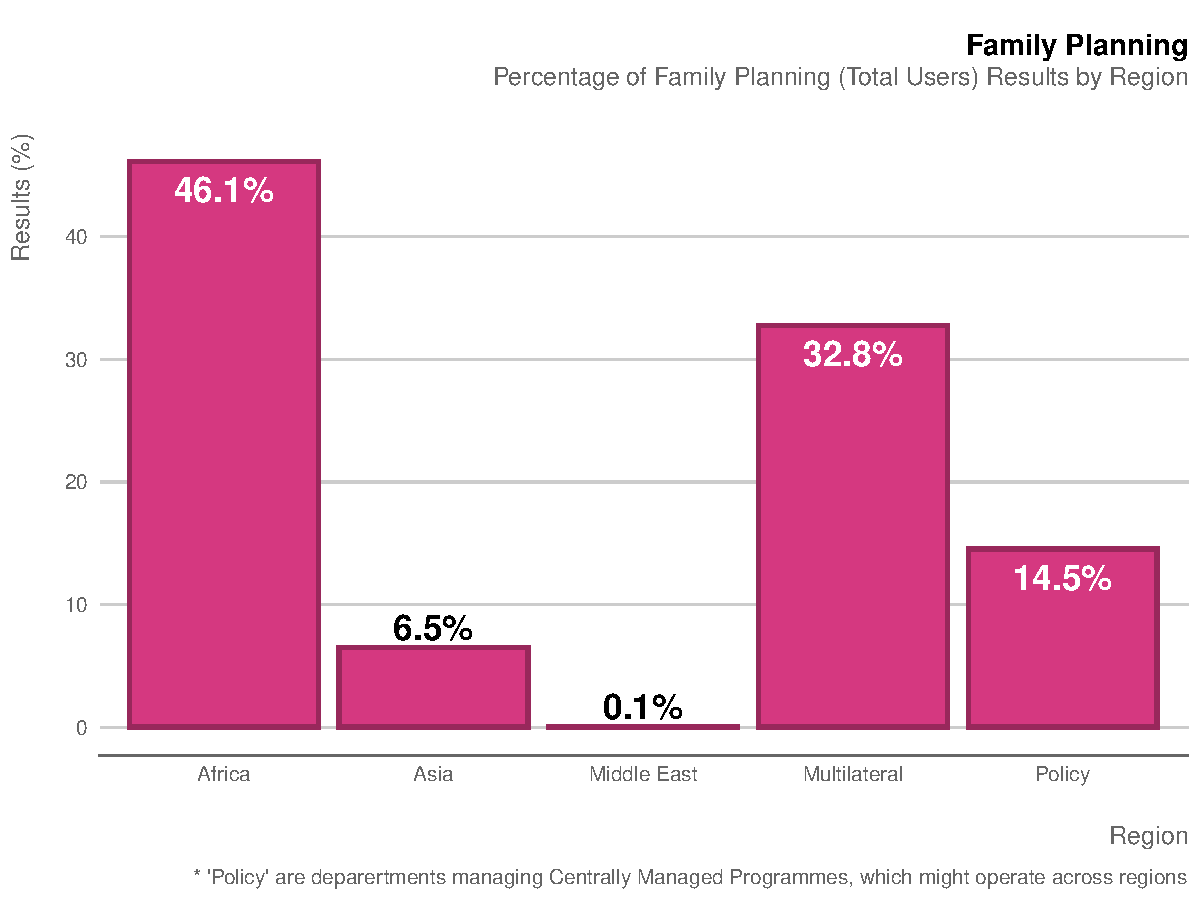
\includegraphics[width=0.8\textwidth]{../figs/fp_total_region_plot} }}%
	\qquad
	\subfloat{{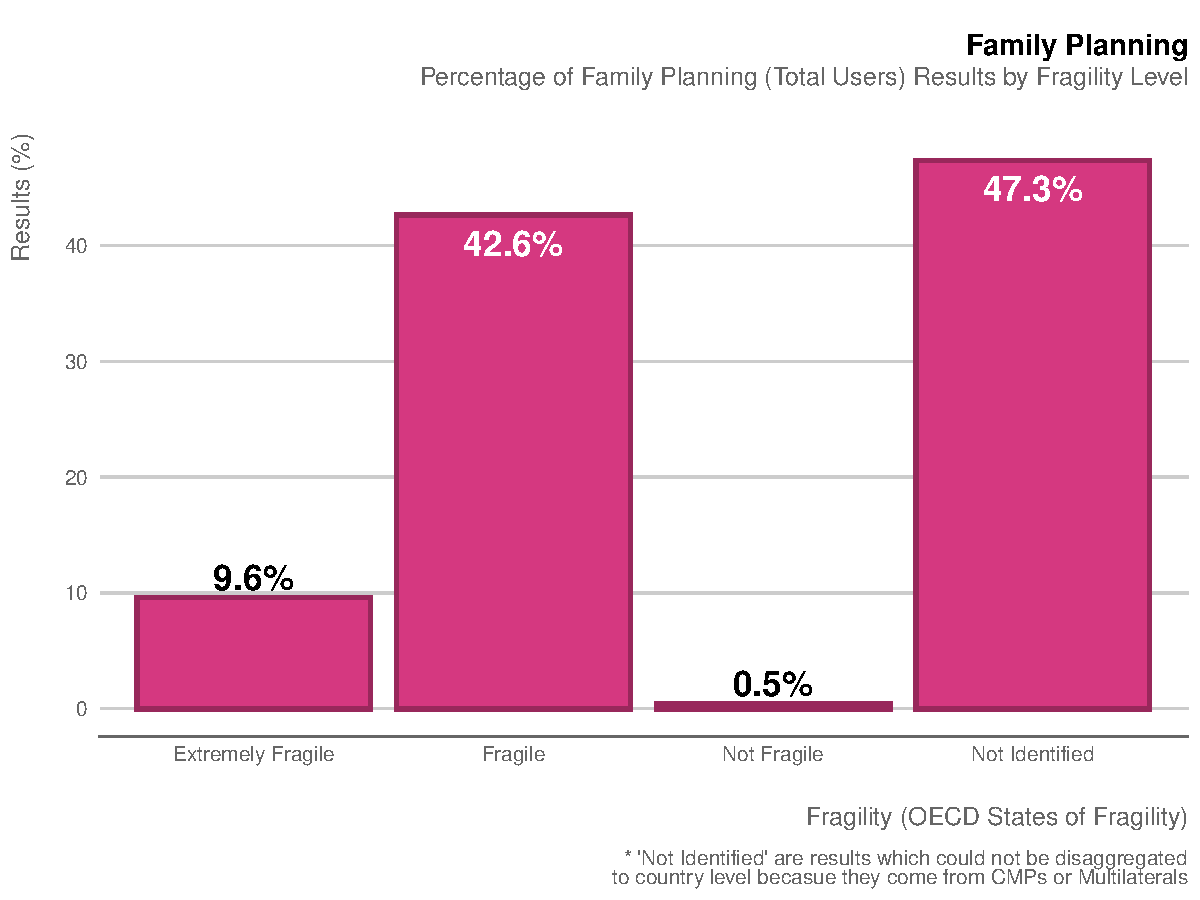
\includegraphics[width=0.8\textwidth]{../figs/fp_total_fragility_plot} }}%
	\caption{Percentage of Family Planning (Total) results by region and fragility level}%
	\label{fig:family_total}
\end{figure}

Between July 2012 and March 2020 DFID reached \textbf{
16.7 million
} \textbf{additional} women and girls with modern methods of family planning. %

Between April 2012 and March 2018, DFID spent an average of \pounds 193.6 million (approx.) on Family Planning every year. %

Between April 2017 and March 2018, DFID spent \pounds 241.5 million on Family Planning\footnote{\href{http://www.who.int/mediacentre/factsheets/fs351/en/}{http://www.who.int/mediacentre/factsheets/fs351/en/}}. %

% not generated in chunk
\begin{figure}
	\centering
	\subfloat{{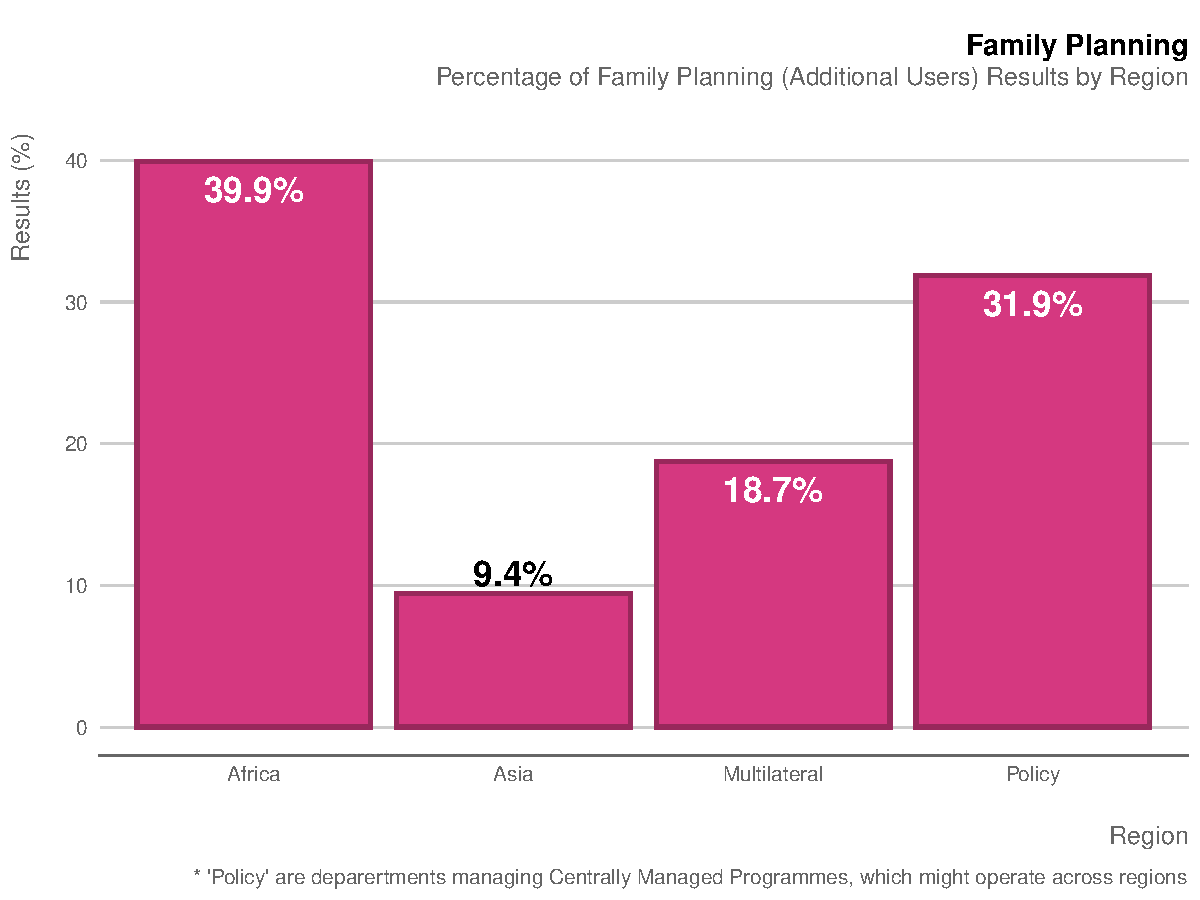
\includegraphics[width=0.8\textwidth]{../figs/fp_additional_region_plot} }}%
	\qquad
	\subfloat{{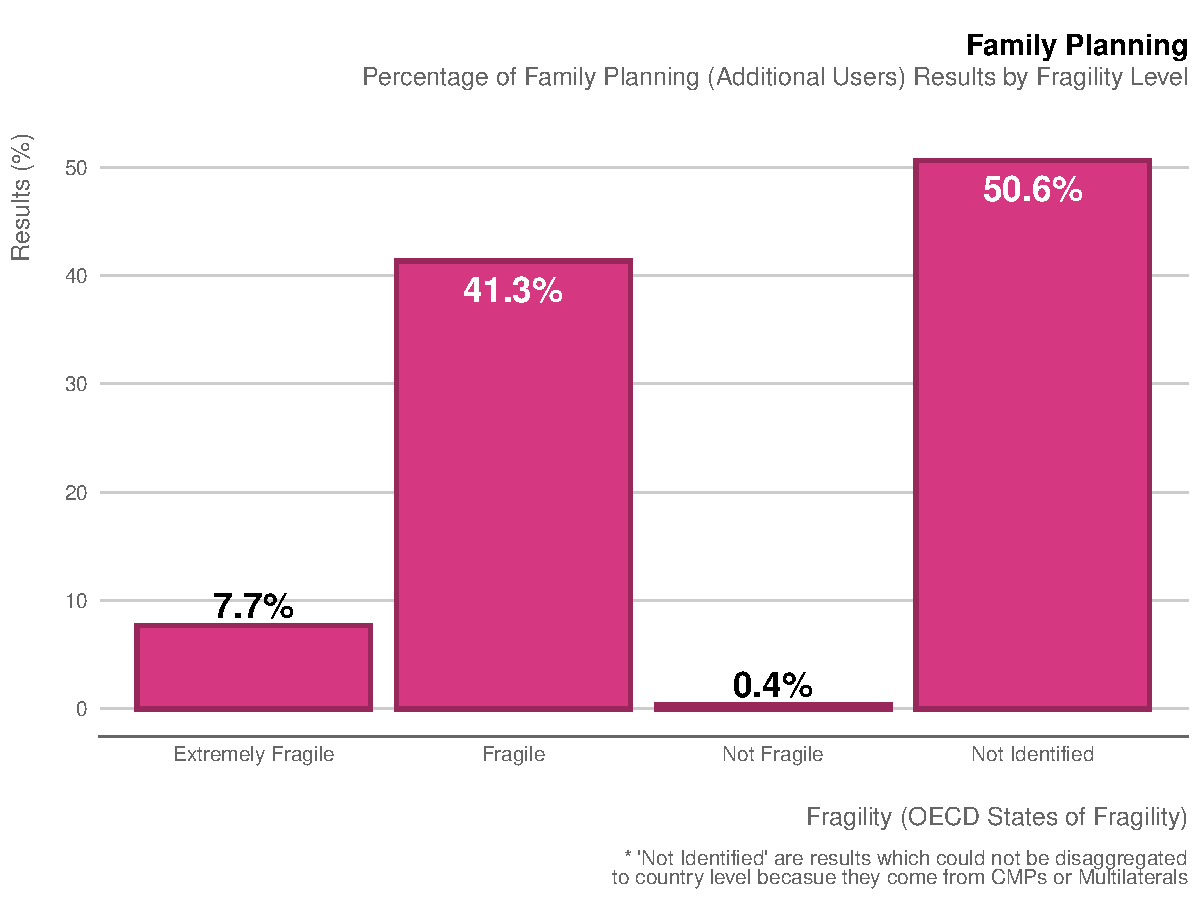
\includegraphics[width=0.8\textwidth]{../figs/fp_additional_fragility_plot} }}%
	\caption{Percentage of Family Planning (Additional) results by region and fragility level}
	\label{fig:family_additional}
\end{figure}


\section{Context}

Family planning is a major pillar of DFID's support to comprehensive Sexual and Reproductive Health and Rights. %
Family planning information, services and supplies enable women and girls to decide whether to have children, when and how many and to determine the spacing of pregnancies and is achieved via the use of modern contraceptive methods\footnote{\href{https://www.guttmacher.org/fact-sheet/adding-it-up-investing-in-sexual-reproductive-health}{https://www.guttmacher.org/fact-sheet/adding-it-up-investing-in-sexual-reproductive-health}}. %
This is fundamental to women and girl's empowerment, enabling them to have control over their lives helping to avoid early, multiple and frequently dangerous pregnancies and births, and instead complete their education, take up economic opportunities and fulfil their potential. %
There are an estimated 218 million women and girls, including 14 million adolescents in developing countries who want to time, space or prevent a pregnancy but are not using modern methods of family planning\footnote{\href{https://www.guttmacher.org/fact-sheet/adding-it-up-investing-in-sexual-reproductive-health-adolescents}{https://www.guttmacher.org/fact-sheet/adding-it-up-investing-in-sexual-reproductive-health-adolescents}}\footnote{\href{https://www.guttmacher.org/sites/default/files/report_downloads/adding-it-up-2019-report-appendix-tables.xlsx}{https://www.guttmacher.org/sites/default/files/report\_downloads/adding-it-up-2019-report-appendix-tables.xlsx}}. %
Unintended pregnancies and unsafe abortions would drop by about two-thirds each, and maternal deaths would reduce by more than one-fifth, if all women in developing countries wanting to avoid a pregnancy were to use modern contraceptives. %

Family Planning is one of the best investments in development. %
The Copenhagen Consensus estimated that every \$1 invested in meeting the unmet need for contraceptives yields in the long-term \$120 in accrued annual benefits (based on reduced infant and maternal mortality and long-term benefits from economic growth)\footnote{\href{http://www.familyplanning2020.org/sites/default/files/Data-Hub/ROI/FP2020_ROI_OnePager_FINAL.pdf}{http://www.familyplanning2020.org/sites/default/files/Data-Hub/ROI/FP2020\_ROI\_OnePager\_FINAL.pdf}}. %
Every dollar spent on contraceptive services beyond the current level would save \$3 in the cost of maternal, newborn and abortion care because use of contraceptives reduces the number of unintended pregnancies\footnote{\href{https://www.guttmacher.org/fact-sheet/adding-it-up-investing-in-sexual-reproductive-health}{https://www.guttmacher.org/fact-sheet/adding-it-up-investing-in-sexual-reproductive-health}}. %

The 2012 London Summit on Family Planning, hosted by the UK and the Bill and Melinda Gates Foundation, built on existing initiatives to put family planning higher on the global agenda, set international goals to enable women and girls to choose to use modern contraceptives and established the Family Planning 2020 (FP2020) partnership\footnote{\href{www.familyplanning2020.org}{www.familyplanning2020.org}}. %
The UK is a core convenor of this partnership, the second largest global bilateral donor on family planning, and co-funds the FP2020 Secretariat\footnote{\href{http://www.track20.org/pages/resources/FP2020_annual_reports.php}{http://www.track20.org/pages/resources/FP2020\_annual\_reports.php}}. %
In 2017, the UK co-hosted a follow-up Family Planning Summit with the Bill and Melinda Gates Foundation and UNFPA. %
The summit focused on innovation and tackling the barriers to progress. %
Over 50 countries, as well as civil society organisations, private sector partners and foundations made commitments to accelerate progress\footnote{\href{http://summit2017.familyplanning2020.org/}{http://summit2017.familyplanning2020.org/}}. %

The Department for International Development, UK (DFID) delivers family planning programmes in support of accelerating progress on voluntary family planning in developing countries and the UK's spend commitment. %
DFID funds a wide range of programmes in this area. %
Many support an integrated package of services for reproductive, maternal, newborn and child health through government facilities and the private sector. %
Some programmes provide contraceptives and other key commodities and others include strong aspects of community work to increase demand and change the social norms around accessing family planning. %
Results are tracked across all these different types of programmes using two indicators:
\begin{adjustwidth}{0.5cm}{}
\textbf{Total Users:} This indicator is defined as the number of women and girls who are currently using, or whose sexual partner is currently using at least one method of modern contraception through DFID's support. %
This indicator not only takes into account DFID's support to maintaining existing users of family planning and but also DFID's work to reach to new users of contraception in developing countries\footnote{This term refers to first-time users of contraception and/or users not recently using a method (e.g. a lapsed user)}. %

\medskip

\noindent\textbf{Additional Users:} Additional users are defined as the difference in total family planning users between years. Therefore, this indicator tracks DFID's support to expanding access to family planning in developing countries.%
\end{adjustwidth}


\newpage
